\documentclass{beamer}
\usepackage[utf8]{inputenc}
\usepackage{tabularx}
\usepackage{mathrsfs}
\usepackage{pgf}
\usepackage{amsmath}
\usepackage{array}
\usepackage{pifont}% http://ctan.org/pkg/pifont
\newcommand{\cmark}{\ding{51}}%
\newcommand{\xmark}{\ding{55}}%
% \usepackage{enumitem}
\usepackage[ruled]{algorithm2e}


% \usepackage{algorithm}
\usepackage{algpseudocode}

\usepackage{tikz}
\usetikzlibrary{calc, chains, decorations.pathmorphing}
\usetikzlibrary{shapes.geometric}
\usetikzlibrary{arrows,shapes,positioning}
\usetikzlibrary{calc,decorations.markings}
\usetikzlibrary{decorations.text}
\usetikzlibrary{patterns}
\usetikzlibrary{arrows.meta}
\usepackage{color, soul}


\definecolor{top-darkblue}{RGB}{62,78,99} 
\definecolor{foot-darkblue}{RGB}{77,82,151} 
\definecolor{foot-blue}{RGB}{171,200,230} 
\definecolor{title-blue}{RGB}{0,76,153}

\definecolor{block-red}{rgb}{1.1, 0.41, 0.38}
\definecolor{propa-grey}{rgb}{0.82, 0.84, 0.86}
\definecolor{true-green}{RGB}{182,191,0}%{rgb}{0, 0.8, 0.2}
\definecolor{purple}{rgb}{0.74, 0.2, 0.64}
\definecolor{cons-red}{rgb}{0.5, 0.11, 0.11}

\definecolor{UPMCEngagementBlueA} {RGB}{140,184,198}
\definecolor{UPMCEngagementBlueB} {RGB}{92,127,146}

\definecolor{UPMCCorporateGreen} {RGB}{182,191,0}
\definecolor{UPMCExcellenceOrangeA} {RGB}{224,82,6}
\definecolor{UPMCExcellenceOrangeB} {RGB}{225,160,47}

\mode<presentation> {
  \usetheme[not@ku={UPMC}, wide, TPomitframeno, FTalign=left,%
  greyfoot, fnolabel=, basecolour=UPMCEngagementBlueB,%
  sidebar=0pt]{Frederiksberg}
  \setbeamercolor{block title example}{bg=UPMCCorporateGreen}
  \setbeamercolor{block title alerted}{bg=UPMCExcellenceOrangeA}
  \setbeamercolor{alerted text}{fg=UPMCExcellenceOrangeA}
  \setbeamertemplate{headline}{}
  \setbeamertemplate{footline}[page number]{}
  \setbeamercovered{transparent}
  \beamertemplatenavigationsymbolsempty
}

\definecolor{red}{rgb}{0.7, 0.11, 0.11}
\definecolor{green}{rgb}{0, 0.8, 0.2}

\tikzstyle{point}=[circle,draw,thick,fill=black,scale=0.2]
\tikzstyle{point+}=[circle,draw=red,thick,fill=red,scale=0.3]
\tikzstyle{class2}=[ellipse, draw, minimum width=2cm, minimum height=1cm]
\tikzstyle{class1}=[ellipse, draw, minimum width=1cm, minimum height=1cm]

\tikzstyle{decision}=[circle,draw,thick,fill=UPMCEngagementBlueA]
\tikzstyle{decision-graph}=[text width={width("$\neg x_3@3$")},circle,
align=center,draw,thick,fill=yellow]
\tikzstyle{propa-graph}=[text width={width("$\neg x_3@3$")},circle,draw,thick,
align=center,fill=propa-grey]
\tikzstyle{conflict}=[<->,>=latex,rounded corners=5pt,thick,draw=blue, line width=1mm]
\tikzstyle{uip}=[draw=true-green,ultra thick]
\tikzstyle{cut}=[-,>=stealth,rounded corners=5pt,thick,draw=blue, line width=0.4mm]
\tikzstyle{link}=[->,>=latex,rounded corners=5pt,thick]
\tikzstyle{unsat}=[draw,thick,fill=red]
\tikzstyle{sat}=[draw,thick,fill=green]
\tikzstyle{propa}=[draw,thick,fill=propa-grey]
\tikzstyle{backtrack}=[->,>=latex,dashed,rounded corners=20pt,thick,draw=blue, line width=0.5mm]

\setbeamertemplate{footline}[frame number]{}

% Definition of variable
\def\SAT{\textcolor{green}{\texttt{SAT}}}
\def\UNSAT{\textcolor{red}{\texttt{UNSAT}}}

\def\true{\textcolor{green}{\texttt{true}}}
\def\false{\textcolor{red}{\texttt{false}}}

\def\ok{\textcolor{green}{\cmark}}
\def\ko{\textcolor{red}{\xmark}}



\begin{document}

\author{Hakan \textsc{METIN}}

\begin{frame}
\frametitle{Exploitation des symétries dynamiques pour la résolution des problèmes SAT}
\framesubtitle{Thèse de doctorat de Sorbonne Université}
 
   Hakan \textsc{Metin}\\
  \vfill
  %\begin{center}

	\scriptsize
    \begin{tabular}{ll}
  	    \textbf{Supervisors:} & \\
    	\textsc{Souheib Baarir}  & Maître de conférences, Université Paris Nanterre\\
    	\vspace{1em}
    	\textsc{Fabrice Kordon}  & Professeur, Sorbonne Université\\
 	    \textbf{Jury Members:} & \\
    	\textsc{Pascal \textsc{Fontaine}}  &  Maître de conférences, Université de Lorraine\\
    	\textsc{Laure Petrucci}  & Professeur, Université Paris 13\\
    	\textsc{Jean-Michel	Couvreur}  & Professeur, Université d'Orléans\\
    	\textsc{Emanuelle Encrenaz}  & Maître de conférences, Sorbonne Université\\
    	\textsc{Souheib Baarir}  & Maître de conférences, Université Paris Nanterre\\
    	\textsc{Fabrice Kordon}  & Professeur, Sorbonne Université\\
    \end{tabular}\\
 % \end{center}

  \vskip 3ex
  \begin{columns}[t]
    \begin{column}[T]{\textwidth}
      
\includegraphics[height=1.2cm]{images/logo_sorbonne}
      \hfill
      
\includegraphics[height=1.3cm]{images/lip6}
      \centering
    \end{column}
  \end{columns}
\end{frame}

%% ----------------------------------------------------------------------------
\begin{frame}
  \frametitle{SAT by example: simple planning decision}
  
  \centering
 \begin{tabular}{c|c |c}
 	  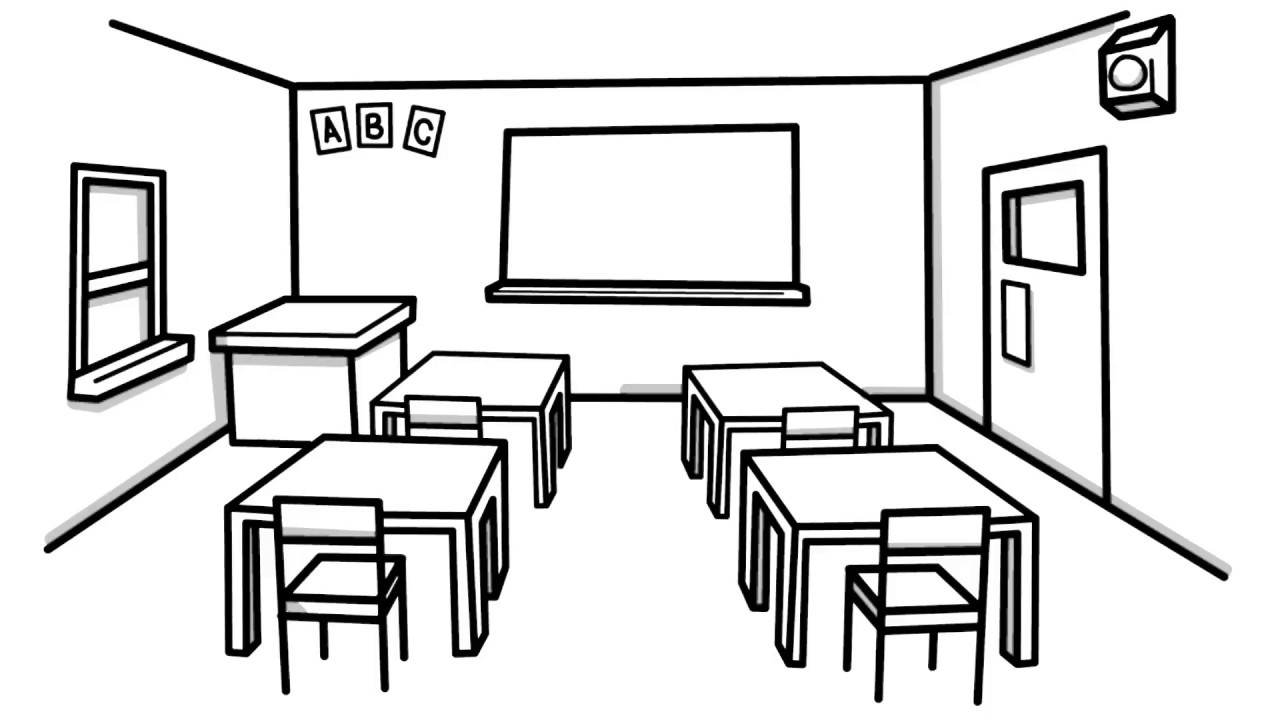
\includegraphics[scale=0.07]{images/room} & 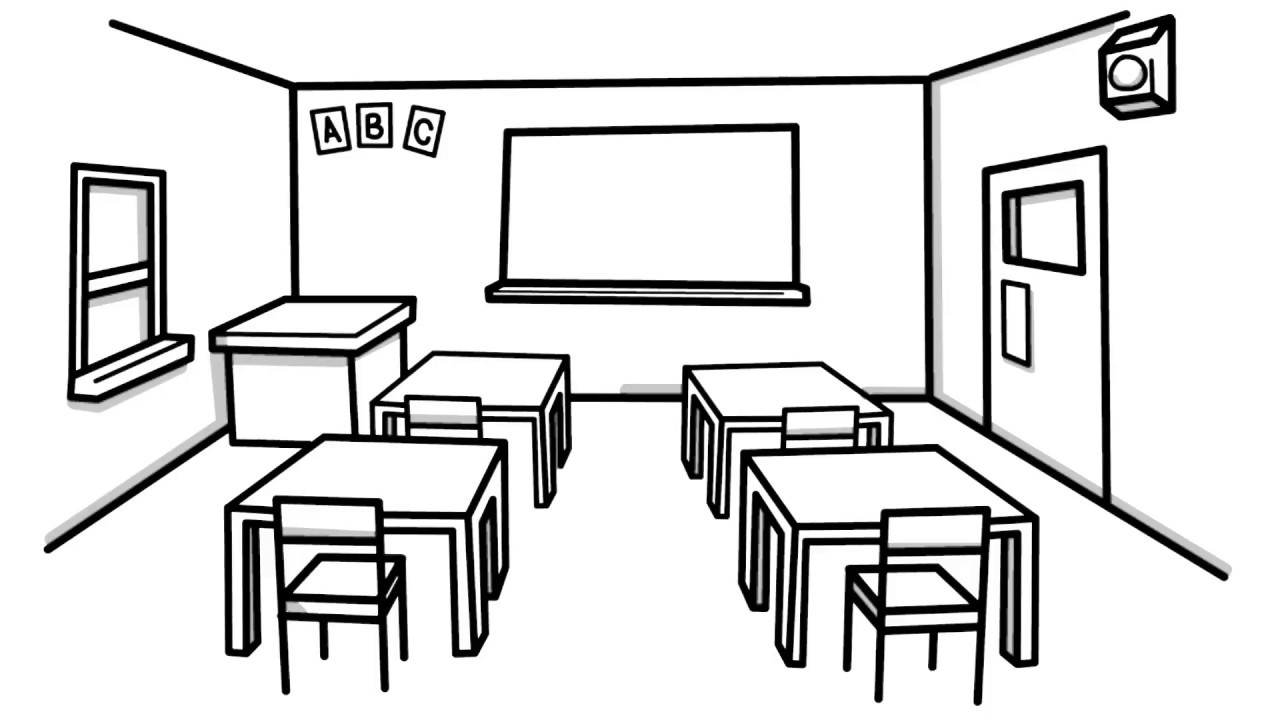
\includegraphics[scale=0.07]{images/room}& 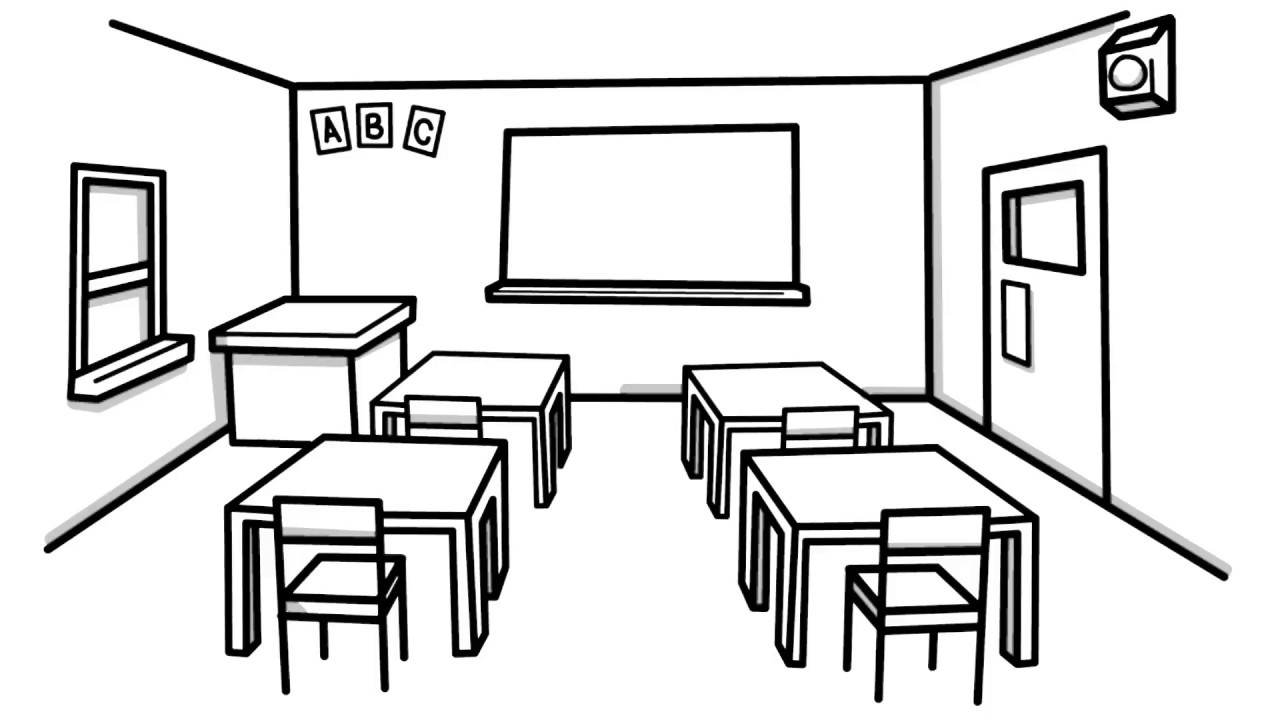
\includegraphics[scale=0.07]{images/room}\\
 	   1                                        & 2                                        & 3\\
 \end{tabular}
\vfill
 \begin{tabular}{c|c|c}
	
\includegraphics[scale=0.1]{images/south} & 
\includegraphics[scale=0.1]{images/simpson} & 
\includegraphics[scale=0.09]{images/titeuf}\\
	 A                                        & B                                           & C\\
\end{tabular}
\vfill
Attribute each group to a class room
\end{frame}
%% ----------------------------------------------------------------------------
\begin{frame}
\frametitle{Encoding the problem}

$(A,1) (A,2) (A,3)$\\
$(B,1) (B,2) (B,3)$\\
$(C,1) (C,2) (C,3)$
\vfill
$ \neg (A,1)  \neg (B,1)$\\
$ \neg (A,1)  \neg (C,1)$\\
$ \neg (B,1)  \neg (C,1)$\\
\vfill
$ \neg (A,2)  \neg (B,2)$\\
$ \neg (A,2)  \neg (C,2)$\\
$ \neg (B,2)  \neg (C,2)$\\
\vfill
$ \neg (A,3)  \neg (B,3)$\\
$ \neg (A,3)  \neg (C,3)$\\
$ \neg (B,3)  \neg (C,3)$\\


%$\omega_1 = x_1 \lor  x_2 \lor x_3 $ \\
%$\omega_2 = x_4 \lor  x_5 \lor x_6 $ \\
%$\omega_3 = x_7 \lor  x_8 \lor x_9 $ \\
%\vfill
%$\omega_4 = \neg x_1 \lor  \neg x_4 $ \\
%$\omega_5 = \neg x_1 \lor  \neg x_7 $ \\
%$\omega_6 = \neg x_4 \lor  \neg x_7 $ \\
%\vfill
%$\omega_7 = \neg x_2 \lor  \neg x_5 $ \\
%$\omega_8 = \neg x_2 \lor  \neg x_8 $ \\
%$\omega_9 = \neg x_5 \lor  \neg x_8 $ \\
%\vfill
%$\omega_{10} = \neg x_3 \lor  \neg x_6 $ \\
%$\omega_{11} = \neg x_3 \lor  \neg x_9 $ \\
%$\omega_{12} = \neg x_6 \lor  \neg x_9 $ \\

\end{frame}
%% ----------------------------------------------------------------------------
\begin{frame}
\frametitle{SAT}
	Algorithm solving 
	CDCL
	
	NP complete problem

\end{frame}
%% ----------------------------------------------------------------------------
\begin{frame}
\frametitle{SAT}
	example solving arbre
	
\end{frame}
%% ----------------------------------------------------------------------------
\begin{frame}
\frametitle{SAT}

\centering
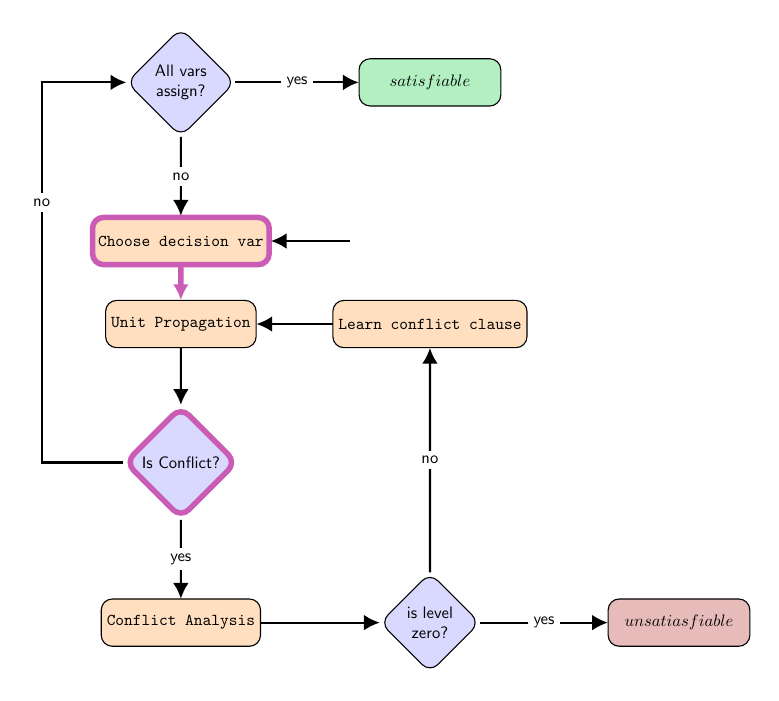
\begin{tikzpicture}[scale=1,every node/.style={scale=0.6,fill=white, font=\sffamily}, align=center]
	% Specification of nodes (position, etc.)
	\tikzset{%	
		>={Latex[width=2mm,length=2mm]},
		% Specifications for style of nodes:
		base/.style = {rectangle, rounded corners, draw=black,
			minimum width=2cm, minimum height=1cm,
			text centered, font=\sffamily},
		question/.style = {base, diamond, fill=blue!15},
		question/.style = {base, diamond, fill=blue!15},
		unsat/.style = {base, fill=red!30,minimum width=3cm},
		sat/.style = {base, fill=green!30,minimum width=3cm},
		process/.style = {base, minimum width=2.5cm, fill=orange!25,
			font=\ttfamily},
		processcurr/.style = {process, thick, line width=0.7mm, draw=purple!80 },
		questioncurr/.style = {question,line width=0.7mm, draw=purple!80},
		line/.style = {->, thick },
		linecurr/.style = {line, line width=0.7mm, draw=purple!80},
	}
	\node (isfin) [question] {All vars\\ assign?};
	\node (dec)     [processcurr, below = of isfin]          {Choose decision var};
	\node (sdec)     [right = of dec]          {};
	\node (idec) [left = of isfin]  {};
	\node (prop)    [process] at ($(dec) + (0pt, -30pt)$)          {Unit Propagation};
	\node (conf)    [questioncurr] at ($(prop) + (0pt, -50pt)$){ Is Conflict?};
	\node (confanalyse) [process, below = of conf] {Conflict Analysis};
	\node (learn) [process] at ($(prop) + (90pt, 0)$) {Learn conflict clause};
	\node (isend) [question] at ($(confanalyse) + (90pt, 0)$) {is level\\zero?};
	\node (end) [unsat] at ($(isend) + (90pt, 0)$) {$unsatiasfiable$};
	\node (ends) [sat] at ($(isfin) + (+90pt, 0)$){$satisfiable$};
	
	\draw[line]     (sdec) -- (dec);
	\draw[linecurr]     (dec) -- (prop);
	\draw[line]     (prop) -- (conf);
	\draw[line]     (conf) -| node [yshift=5.5 cm] {no}(idec.center) -- (isfin);
	\draw[line]     (conf) -- node {yes} (confanalyse);
	\draw[line]     (isfin) -- node {no}(dec);
	\draw[line]     (confanalyse) --(isend);
	\draw[line]     (isend) -- node {yes}(end);
	\draw[line]     (isfin) -- node {yes}(ends);
	\draw[line]     (learn) -- (prop);
	\draw[line]     (isend) -- node [] {no}(learn);	
	\end{tikzpicture}

\end{frame}
%% ----------------------------------------------------------------------------
\begin{frame}
\frametitle{SAT}

\end{frame}

%% ----------------------------------------------------------------------------

\begin{frame}[allowframebreaks,noframenumbering]
  \scriptsize
  \nocite{*}
  \bibliographystyle{alpha}
  \bibliography{main}
\end{frame}


\end{document}